
% TODO: 3.段落が短すぎるのでまとめたり増やす必要がある.
\subsubsection{無線送信機からの受信電波情報と基地局情報を用いた初期進行方向の補正}

マップマッチングによる初期進行方向の補正は,建物の構造に強く依存するため,
オープンスペースが多い環境や廊下などの単純な構造を持つ空間では十分な補正効果が得られない可能性がある.
このような環境下での補正手法として,環境中に設置された無線送信機の基地局情報を活用した初期進行方向補正手法を実装している.
この補正機能は,WirelessSignalCorrectorクラスとして提供しており,建物構造に依存せず初期進行方向の推定が可能である.

WirelessSignalCorrectorクラスの利用例をListing\ref{lst:ble-beacon-position}に示す.
このクラスを利用するために必要な情報は主に2つある.1つ目は歩行者が
移動中に収集した信号スキャンデータである.これは歩行者の
スマートフォンが周辺の無線送信機を検知した際に記録される情報で,
各送信機のID,検知した時刻,そのときの電波強度(RSSI)が含まれている.
歩行者が送信機に近づいたり遠ざかると,この電波強度は
時間とともに変化する.2つ目は送信機の基地局情報である.
これは各送信機のIDとその送信機が実際に設置されている座標が
記録された情報である.図\ref{fig:ble-beacon-position}は,
xDR Challenge 2023環境におけるBLEビーコンの配置例を示している.各送信機は
既知の座標に固定されており,歩行者の移動に伴って受信されるRSSI値が変化する.
% TODO:手法なのかクラスなのか統一しよう

% TODO: 2.データが1つしかないように見える.複数個あるのを表現した方がいいと思う.
% TODO: 2.captionの名前は検討した方がいいかも
\begin{lstlisting}[caption={WirelessSignalCorrectorの使用例},label=lst:ble-beacon-position,float=h]
# 送信機の基地局情報
transmitter_positions = pd.read_csv('transmitter_positions.csv')
# transmitter_id: "f2:65:d1:87:a4:2c"
# x: 15.2  # メートル
# y: 24.8  # メートル
# floor: "floor_5"

# 歩行中に収集したスキャンデータ
signal_realtime_scans = pd.read_csv('signal_scans.csv')
# ts: 1234567890.123  # タイムスタンプ(秒)
# transmitter_id: "f2:65:d1:87:a4:2c"  # 送信機ID
# rssi: -68  # 電波強度(dBm)

# WirelessSignalCorrectorの初期化と補正の実行
wireless_corrector = WirelessSignalCorrector(
    signal_realtime_scans=signal_realtime_scans,
    transmitter_positions=transmitter_positions,
    rssi_threshold=-70  # 電波強度の閾値(dBm)
)
\end{lstlisting}

\begin{figure}[H]
    \centering
    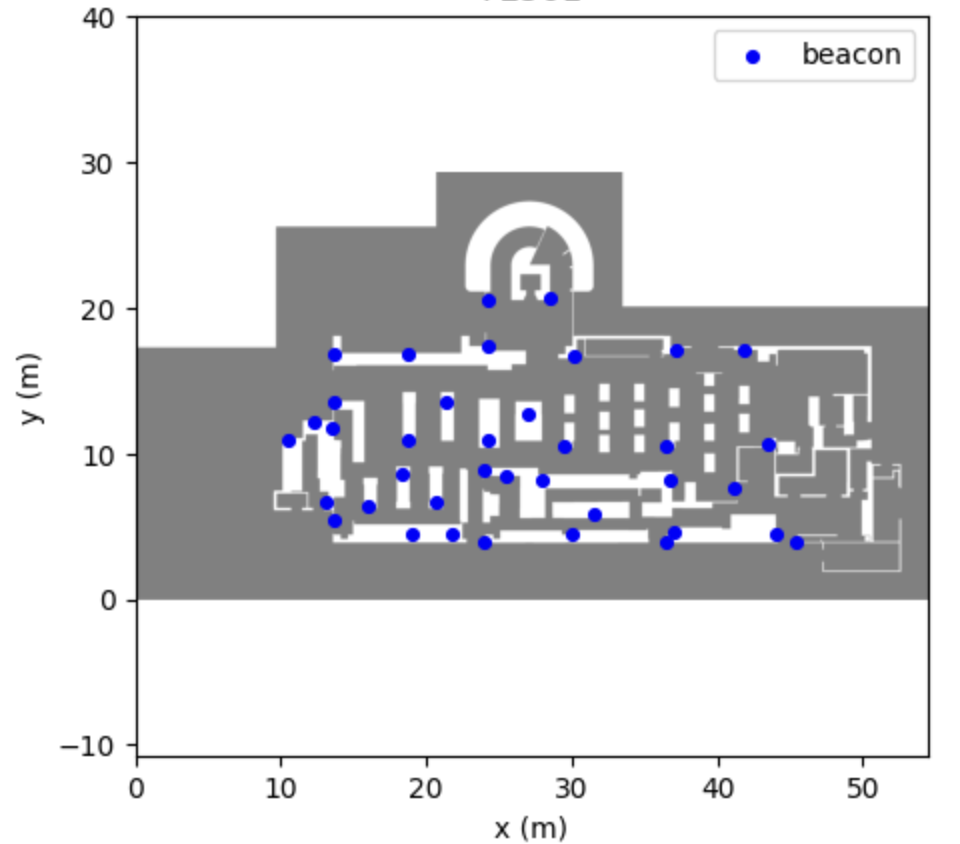
\includegraphics[width=\linewidth]{../image/ble-beacon-position.jpg}
    \caption{送信機(BLEビーコン)の配置例(xDR Challenge 2023環境)}    \label{fig:ble-beacon-position}
\end{figure}

% TODO: 2.RSSIの値はデータの上位何%という風に決めた方がいいかも.
% 多くのビーコンを使用してなんとなくの全体像を把握するの重要なポイントな気がする

WirelessSignalCorrectorのBLE基地局位置を用いた補正処理では,まず受信したスキャンデータに対して閾値処理を行い,RSSI値が閾値を超える受信時刻の集合$T$を定義する.
デフォルトではRSSIが-70dBmより強い信号のみを使用する.この値は一般的な無線信号の減衰特性を考慮して設定されており,およそ3メートル程度の範囲内での受信信号に相当する.
この閾値は環境やユースケースに応じて調整可能であり,WirelessSignalCorrectorの初期化時にrssi\_thresholdパラメータとして指定できる.
例えば与えられる信号スキャンデータの電波強度が強い割合が小さい場合は-80dBm程度に緩和し,逆に割合が多い場合は-65dBm程度に厳格化するといった調整が可能である.

集合$T$に含まれる各受信時刻$t$について,推定軌跡上のもっとも近い時刻のポイントを特定する.
図\ref{fig:ble-merge}は,この対応付けの結果を可視化したものである.
軌跡上のポイントは時間経過に応じて色付けされており,青色のポイントは対応するBLE基地局の位置を示している.
各受信時刻$t$における軌跡上の点と対応するBLE基地局との距離の総和$D(\theta)$を式\eqref{eq:distance_sum}で定義する.
ここで$(x_t(\theta), y_t(\theta))$は角度$\theta$で回転させた軌跡上の時刻$t$における座標,$(b_x^t, b_y^t)$は時刻$t$で受信したBLE基地局の座標を表す.
最適な回転角度$\theta_{\mathrm{opt}}$は式\eqref{eq:opt}に示すように,距離の総和$D(\theta)$を最小化する角度として定義される.この最適化問題はグリッドサーチにより$[0, 2\pi]$の範囲で解を探索する.
BLE基地局の位置と推定軌跡の位置関係がもっとも整合する角度を見つけ,最適な初期進行方向を決定できる.

この手法の特徴は建物の構造に依存せず,基地局が適切に配置されていれば任意の環境で適用可能な点にある.
また電波強度の閾値の調整によって補正の精度と信頼性のバランスを制御できる.
閾値を下げた場合より多くの信号を用いて補正を行えるが,信頼性の低い信号も含まれる可能性が高くなる.
逆に閾値を上げた場合信頼性は高くなるが,使用可能な信号数が減少する.
ただしこの手法の効果は基地局の配置密度や,環境内での電波伝搬特性に影響される点には注意が必要である.
特に,基地局が一様に配置されていない場合や,遮蔽物により電波が大きく減衰する環境では,補正精度が低下する可能性がある.

\begin{equation}
\label{eq:distance_sum}
D(\theta) = \sum_{t\in T} \sqrt{(x_t(\theta) - b^t_x)^2 + (y_t(\theta) - b^t_y)^2}
\end{equation}

\begin{equation}
\label{eq:opt}
\theta_{\mathrm{opt}} = \arg\min_{\theta \in [0, 2\pi]} D(\theta)
\end{equation}

\begin{figure}[H]
	\centering
	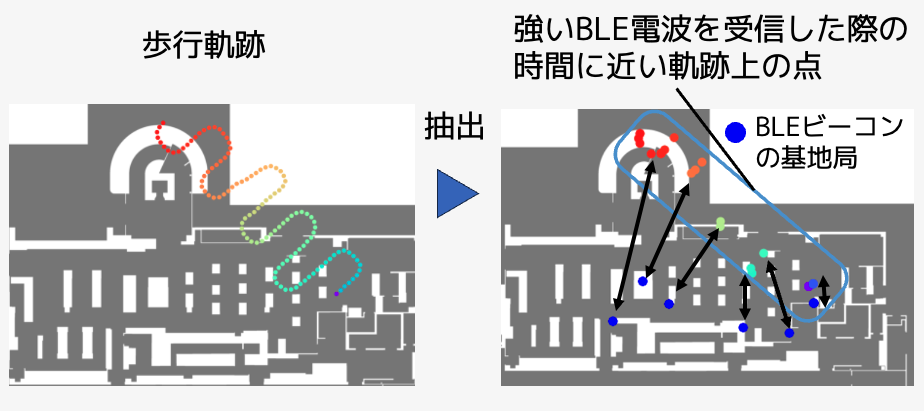
\includegraphics[width=\linewidth]{../image/ble-merge.jpg}
	\caption{BLEビーコンの基地局の基地局情報}    \label{fig:ble-merge}
\end{figure}
